\section{Wm4::Vector3$<$ Real $>$ Class Template Reference}
\label{classWm4_1_1Vector3}\index{Wm4::Vector3@{Wm4::Vector3}}
{\tt \#include $<$Wm4Vector3.h$>$}

Collaboration diagram for Wm4::Vector3$<$ Real $>$:\begin{figure}[H]
\begin{center}
\leavevmode
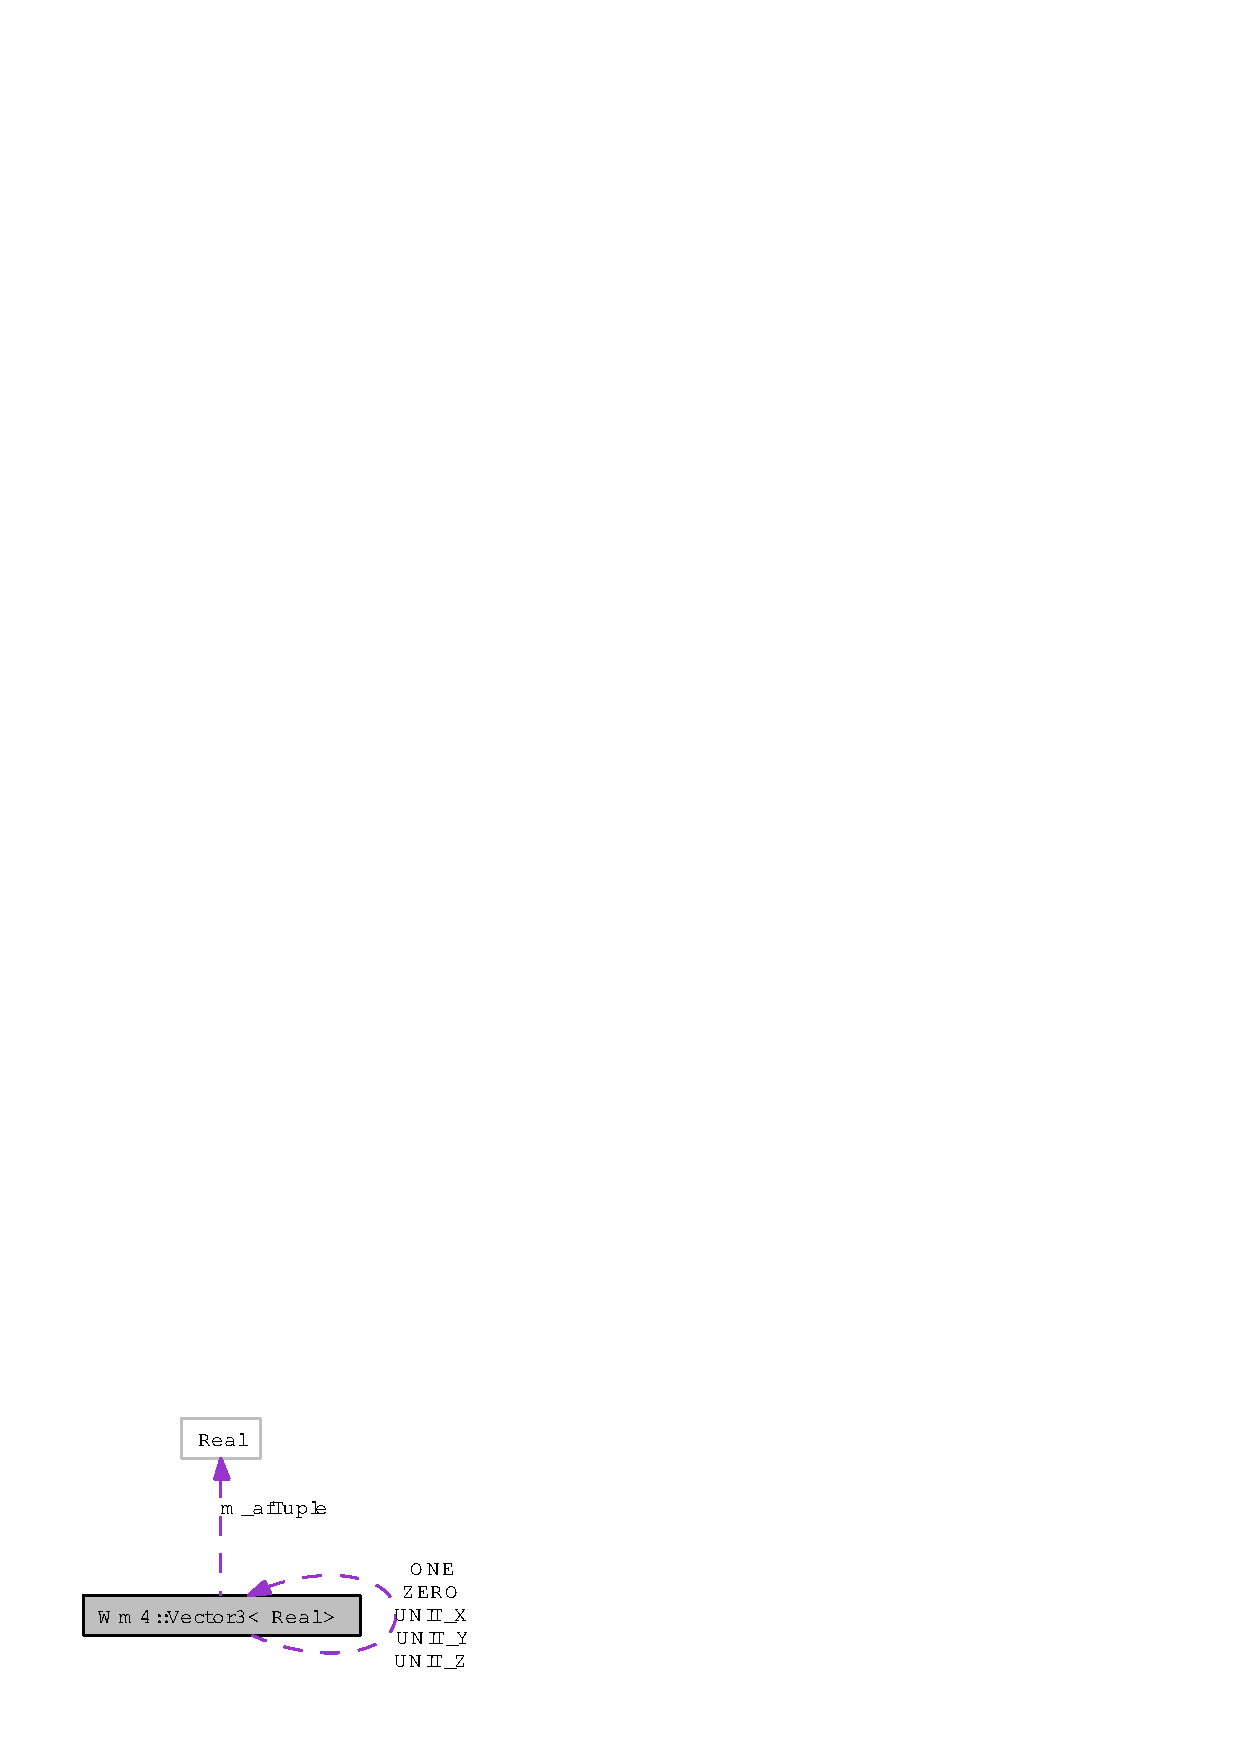
\includegraphics[width=115pt]{classWm4_1_1Vector3__coll__graph}
\end{center}
\end{figure}
\subsection*{Public Member Functions}
\begin{CompactItemize}
\item 
{\bf Vector3} ()
\item 
{\bf Vector3} (Real f\-X, Real f\-Y, Real f\-Z)
\item 
{\bf Vector3} (const Real $\ast$af\-Tuple)
\item 
{\bf Vector3} (const {\bf Vector3} \&rk\-V)
\item 
{\bf operator const Real $\ast$} () const
\item 
{\bf operator Real $\ast$} ()
\item 
Real {\bf operator[$\,$]} (int i) const
\item 
Real \& {\bf operator[$\,$]} (int i)
\item 
Real {\bf X} () const
\item 
Real \& {\bf X} ()
\item 
Real {\bf Y} () const
\item 
Real \& {\bf Y} ()
\item 
Real {\bf Z} () const
\item 
Real \& {\bf Z} ()
\item 
{\bf Vector3} \& {\bf operator=} (const {\bf Vector3} \&rk\-V)
\item 
bool {\bf operator==} (const {\bf Vector3} \&rk\-V) const
\item 
bool {\bf operator!=} (const {\bf Vector3} \&rk\-V) const
\item 
bool {\bf operator$<$} (const {\bf Vector3} \&rk\-V) const
\item 
bool {\bf operator$<$=} (const {\bf Vector3} \&rk\-V) const
\item 
bool {\bf operator$>$} (const {\bf Vector3} \&rk\-V) const
\item 
bool {\bf operator$>$=} (const {\bf Vector3} \&rk\-V) const
\item 
{\bf Vector3} {\bf operator+} (const {\bf Vector3} \&rk\-V) const
\item 
{\bf Vector3} {\bf operator-} (const {\bf Vector3} \&rk\-V) const
\item 
{\bf Vector3} {\bf operator $\ast$} (Real f\-Scalar) const 
\item 
{\bf Vector3} {\bf operator/} (Real f\-Scalar) const 
\item 
{\bf Vector3} {\bf operator-} () const
\item 
{\bf Vector3} \& {\bf operator+=} (const {\bf Vector3} \&rk\-V)
\item 
{\bf Vector3} \& {\bf operator-=} (const {\bf Vector3} \&rk\-V)
\item 
{\bf Vector3} \& {\bf operator $\ast$=} (Real f\-Scalar)
\item 
{\bf Vector3} \& {\bf operator/=} (Real f\-Scalar)
\item 
Real {\bf Length} () const
\item 
Real {\bf Squared\-Length} () const
\item 
Real {\bf Dot} (const {\bf Vector3} \&rk\-V) const
\item 
Real {\bf Normalize} ()
\item 
{\bf Vector3} {\bf Cross} (const {\bf Vector3} \&rk\-V) const
\item 
{\bf Vector3} {\bf Unit\-Cross} (const {\bf Vector3} \&rk\-V) const
\item 
void {\bf Get\-Barycentrics} (const {\bf Vector3} \&rk\-V0, const {\bf Vector3} \&rk\-V1, const {\bf Vector3} \&rk\-V2, const {\bf Vector3} \&rk\-V3, Real af\-Bary[4]) const
\end{CompactItemize}
\subsection*{Static Public Member Functions}
\begin{CompactItemize}
\item 
static void {\bf Orthonormalize} ({\bf Vector3} \&rk\-U, {\bf Vector3} \&rk\-V, {\bf Vector3} \&rk\-W)
\item 
static void {\bf Orthonormalize} ({\bf Vector3} $\ast$ak\-V)
\item 
static void {\bf Generate\-Orthonormal\-Basis} ({\bf Vector3} \&rk\-U, {\bf Vector3} \&rk\-V, {\bf Vector3} \&rk\-W)
\item 
static void {\bf Generate\-Complement\-Basis} ({\bf Vector3} \&rk\-U, {\bf Vector3} \&rk\-V, const {\bf Vector3} \&rk\-W)
\item 
static void {\bf Compute\-Extremes} (int i\-VQuantity, const {\bf Vector3} $\ast$ak\-Point, {\bf Vector3} \&rk\-Min, {\bf Vector3} \&rk\-Max)
\end{CompactItemize}
\subsection*{Static Public Attributes}
\begin{CompactItemize}
\item 
static WM4\_\-FOUNDATION\_\-ITEM const {\bf Vector3} {\bf ZERO}
\item 
static WM4\_\-FOUNDATION\_\-ITEM const {\bf Vector3} {\bf UNIT\_\-X}
\item 
static WM4\_\-FOUNDATION\_\-ITEM const {\bf Vector3} {\bf UNIT\_\-Y}
\item 
static WM4\_\-FOUNDATION\_\-ITEM const {\bf Vector3} {\bf UNIT\_\-Z}
\item 
static WM4\_\-FOUNDATION\_\-ITEM const {\bf Vector3} {\bf ONE}
\end{CompactItemize}
\subsubsection*{template$<$class Real$>$ class Wm4::Vector3$<$ Real $>$}



\subsection{Constructor \& Destructor Documentation}
\index{Wm4::Vector3@{Wm4::Vector3}!Vector3@{Vector3}}
\index{Vector3@{Vector3}!Wm4::Vector3@{Wm4::Vector3}}
\subsubsection{\setlength{\rightskip}{0pt plus 5cm}template$<$class Real$>$ {\bf Wm4::Vector3}$<$ Real $>$::{\bf Vector3} ()}\label{classWm4_1_1Vector3_0be5457c1a2ed752bd762a343fff6966}


\index{Wm4::Vector3@{Wm4::Vector3}!Vector3@{Vector3}}
\index{Vector3@{Vector3}!Wm4::Vector3@{Wm4::Vector3}}
\subsubsection{\setlength{\rightskip}{0pt plus 5cm}template$<$class Real$>$ {\bf Wm4::Vector3}$<$ Real $>$::{\bf Vector3} (Real {\em f\-X}, Real {\em f\-Y}, Real {\em f\-Z})}\label{classWm4_1_1Vector3_c447f97781c24e59be04539611a59e56}


\index{Wm4::Vector3@{Wm4::Vector3}!Vector3@{Vector3}}
\index{Vector3@{Vector3}!Wm4::Vector3@{Wm4::Vector3}}
\subsubsection{\setlength{\rightskip}{0pt plus 5cm}template$<$class Real$>$ {\bf Wm4::Vector3}$<$ Real $>$::{\bf Vector3} (const Real $\ast$ {\em af\-Tuple})}\label{classWm4_1_1Vector3_1c8c298fef9dacf92a789178878d4803}


\index{Wm4::Vector3@{Wm4::Vector3}!Vector3@{Vector3}}
\index{Vector3@{Vector3}!Wm4::Vector3@{Wm4::Vector3}}
\subsubsection{\setlength{\rightskip}{0pt plus 5cm}template$<$class Real$>$ {\bf Wm4::Vector3}$<$ Real $>$::{\bf Vector3} (const {\bf Vector3}$<$ Real $>$ \& {\em rk\-V})}\label{classWm4_1_1Vector3_e231716c3dd5d198ad17ef0c55cdd90b}




\subsection{Member Function Documentation}
\index{Wm4::Vector3@{Wm4::Vector3}!operator const Real *@{operator const Real $\ast$}}
\index{operator const Real *@{operator const Real $\ast$}!Wm4::Vector3@{Wm4::Vector3}}
\subsubsection{\setlength{\rightskip}{0pt plus 5cm}template$<$class Real$>$ {\bf Wm4::Vector3}$<$ Real $>$::operator const Real $\ast$ () const\hspace{0.3cm}{\tt  [inline]}}\label{classWm4_1_1Vector3_55e31edc3b1cf7fd110ec88b09863829}


\index{Wm4::Vector3@{Wm4::Vector3}!operator Real *@{operator Real $\ast$}}
\index{operator Real *@{operator Real $\ast$}!Wm4::Vector3@{Wm4::Vector3}}
\subsubsection{\setlength{\rightskip}{0pt plus 5cm}template$<$class Real$>$ {\bf Wm4::Vector3}$<$ Real $>$::operator Real $\ast$ ()\hspace{0.3cm}{\tt  [inline]}}\label{classWm4_1_1Vector3_496ff7239bd1c34d7094ad0d963baf94}


\index{Wm4::Vector3@{Wm4::Vector3}!operator[]@{operator[]}}
\index{operator[]@{operator[]}!Wm4::Vector3@{Wm4::Vector3}}
\subsubsection{\setlength{\rightskip}{0pt plus 5cm}template$<$class Real$>$ Real {\bf Wm4::Vector3}$<$ Real $>$::operator[$\,$] (int {\em i}) const\hspace{0.3cm}{\tt  [inline]}}\label{classWm4_1_1Vector3_3a1e926dc747b7ba08728e2b89348618}


\index{Wm4::Vector3@{Wm4::Vector3}!operator[]@{operator[]}}
\index{operator[]@{operator[]}!Wm4::Vector3@{Wm4::Vector3}}
\subsubsection{\setlength{\rightskip}{0pt plus 5cm}template$<$class Real$>$ Real \& {\bf Wm4::Vector3}$<$ Real $>$::operator[$\,$] (int {\em i})\hspace{0.3cm}{\tt  [inline]}}\label{classWm4_1_1Vector3_f16c1aab5c89b902d4c374fd8ab18f73}


\index{Wm4::Vector3@{Wm4::Vector3}!X@{X}}
\index{X@{X}!Wm4::Vector3@{Wm4::Vector3}}
\subsubsection{\setlength{\rightskip}{0pt plus 5cm}template$<$class Real$>$ Real {\bf Wm4::Vector3}$<$ Real $>$::X () const\hspace{0.3cm}{\tt  [inline]}}\label{classWm4_1_1Vector3_3854b82c9d1ebea73073c5a523abde3b}


\index{Wm4::Vector3@{Wm4::Vector3}!X@{X}}
\index{X@{X}!Wm4::Vector3@{Wm4::Vector3}}
\subsubsection{\setlength{\rightskip}{0pt plus 5cm}template$<$class Real$>$ Real \& {\bf Wm4::Vector3}$<$ Real $>$::X ()\hspace{0.3cm}{\tt  [inline]}}\label{classWm4_1_1Vector3_a63221cc2c958bdda340a7f7f08da6a8}


\index{Wm4::Vector3@{Wm4::Vector3}!Y@{Y}}
\index{Y@{Y}!Wm4::Vector3@{Wm4::Vector3}}
\subsubsection{\setlength{\rightskip}{0pt plus 5cm}template$<$class Real$>$ Real {\bf Wm4::Vector3}$<$ Real $>$::Y () const\hspace{0.3cm}{\tt  [inline]}}\label{classWm4_1_1Vector3_4d9580d763d3710cb58316d769daa6a9}


\index{Wm4::Vector3@{Wm4::Vector3}!Y@{Y}}
\index{Y@{Y}!Wm4::Vector3@{Wm4::Vector3}}
\subsubsection{\setlength{\rightskip}{0pt plus 5cm}template$<$class Real$>$ Real \& {\bf Wm4::Vector3}$<$ Real $>$::Y ()\hspace{0.3cm}{\tt  [inline]}}\label{classWm4_1_1Vector3_ed0ce037680d2e5c19df316d620b19f8}


\index{Wm4::Vector3@{Wm4::Vector3}!Z@{Z}}
\index{Z@{Z}!Wm4::Vector3@{Wm4::Vector3}}
\subsubsection{\setlength{\rightskip}{0pt plus 5cm}template$<$class Real$>$ Real {\bf Wm4::Vector3}$<$ Real $>$::Z () const\hspace{0.3cm}{\tt  [inline]}}\label{classWm4_1_1Vector3_69fce1c602b0b8568d41d05a3ef4088b}


\index{Wm4::Vector3@{Wm4::Vector3}!Z@{Z}}
\index{Z@{Z}!Wm4::Vector3@{Wm4::Vector3}}
\subsubsection{\setlength{\rightskip}{0pt plus 5cm}template$<$class Real$>$ Real \& {\bf Wm4::Vector3}$<$ Real $>$::Z ()\hspace{0.3cm}{\tt  [inline]}}\label{classWm4_1_1Vector3_792db4bd00e018eea9d3be13506b6558}


\index{Wm4::Vector3@{Wm4::Vector3}!operator=@{operator=}}
\index{operator=@{operator=}!Wm4::Vector3@{Wm4::Vector3}}
\subsubsection{\setlength{\rightskip}{0pt plus 5cm}template$<$class Real$>$ {\bf Vector3}$<$ Real $>$ \& {\bf Wm4::Vector3}$<$ Real $>$::operator= (const {\bf Vector3}$<$ Real $>$ \& {\em rk\-V})\hspace{0.3cm}{\tt  [inline]}}\label{classWm4_1_1Vector3_4c462b662e2453a855d2216ae00d4eb1}


\index{Wm4::Vector3@{Wm4::Vector3}!operator==@{operator==}}
\index{operator==@{operator==}!Wm4::Vector3@{Wm4::Vector3}}
\subsubsection{\setlength{\rightskip}{0pt plus 5cm}template$<$class Real$>$ bool {\bf Wm4::Vector3}$<$ Real $>$::operator== (const {\bf Vector3}$<$ Real $>$ \& {\em rk\-V}) const}\label{classWm4_1_1Vector3_f627f662808c5603863d2d7c4202c60a}


\index{Wm4::Vector3@{Wm4::Vector3}!operator"!=@{operator"!=}}
\index{operator"!=@{operator"!=}!Wm4::Vector3@{Wm4::Vector3}}
\subsubsection{\setlength{\rightskip}{0pt plus 5cm}template$<$class Real$>$ bool {\bf Wm4::Vector3}$<$ Real $>$::operator!= (const {\bf Vector3}$<$ Real $>$ \& {\em rk\-V}) const}\label{classWm4_1_1Vector3_397a06523c9a33ca92ccf5c3edd172d5}


\index{Wm4::Vector3@{Wm4::Vector3}!operator<@{operator$<$}}
\index{operator<@{operator$<$}!Wm4::Vector3@{Wm4::Vector3}}
\subsubsection{\setlength{\rightskip}{0pt plus 5cm}template$<$class Real$>$ bool {\bf Wm4::Vector3}$<$ Real $>$::operator$<$ (const {\bf Vector3}$<$ Real $>$ \& {\em rk\-V}) const}\label{classWm4_1_1Vector3_3e9a9c63a62a44e5745aeb9071bf4f55}


\index{Wm4::Vector3@{Wm4::Vector3}!operator<=@{operator$<$=}}
\index{operator<=@{operator$<$=}!Wm4::Vector3@{Wm4::Vector3}}
\subsubsection{\setlength{\rightskip}{0pt plus 5cm}template$<$class Real$>$ bool {\bf Wm4::Vector3}$<$ Real $>$::operator$<$= (const {\bf Vector3}$<$ Real $>$ \& {\em rk\-V}) const}\label{classWm4_1_1Vector3_7800f2c726bd9eb09892f767cd7aba19}


\index{Wm4::Vector3@{Wm4::Vector3}!operator>@{operator$>$}}
\index{operator>@{operator$>$}!Wm4::Vector3@{Wm4::Vector3}}
\subsubsection{\setlength{\rightskip}{0pt plus 5cm}template$<$class Real$>$ bool {\bf Wm4::Vector3}$<$ Real $>$::operator$>$ (const {\bf Vector3}$<$ Real $>$ \& {\em rk\-V}) const}\label{classWm4_1_1Vector3_023cea9ce14058000639c93290ca4295}


\index{Wm4::Vector3@{Wm4::Vector3}!operator>=@{operator$>$=}}
\index{operator>=@{operator$>$=}!Wm4::Vector3@{Wm4::Vector3}}
\subsubsection{\setlength{\rightskip}{0pt plus 5cm}template$<$class Real$>$ bool {\bf Wm4::Vector3}$<$ Real $>$::operator$>$= (const {\bf Vector3}$<$ Real $>$ \& {\em rk\-V}) const}\label{classWm4_1_1Vector3_4854e5f3f495c178e471cda42d896224}


\index{Wm4::Vector3@{Wm4::Vector3}!operator+@{operator+}}
\index{operator+@{operator+}!Wm4::Vector3@{Wm4::Vector3}}
\subsubsection{\setlength{\rightskip}{0pt plus 5cm}template$<$class Real$>$ {\bf Vector3}$<$ Real $>$ {\bf Wm4::Vector3}$<$ Real $>$::operator+ (const {\bf Vector3}$<$ Real $>$ \& {\em rk\-V}) const\hspace{0.3cm}{\tt  [inline]}}\label{classWm4_1_1Vector3_e771fc04c155a10e188bcf2e2b957676}


\index{Wm4::Vector3@{Wm4::Vector3}!operator-@{operator-}}
\index{operator-@{operator-}!Wm4::Vector3@{Wm4::Vector3}}
\subsubsection{\setlength{\rightskip}{0pt plus 5cm}template$<$class Real$>$ {\bf Vector3}$<$ Real $>$ {\bf Wm4::Vector3}$<$ Real $>$::operator- (const {\bf Vector3}$<$ Real $>$ \& {\em rk\-V}) const\hspace{0.3cm}{\tt  [inline]}}\label{classWm4_1_1Vector3_fd35acae902bdf5171c4ae77ecee371e}


\index{Wm4::Vector3@{Wm4::Vector3}!operator *@{operator $\ast$}}
\index{operator *@{operator $\ast$}!Wm4::Vector3@{Wm4::Vector3}}
\subsubsection{\setlength{\rightskip}{0pt plus 5cm}template$<$class Real$>$ {\bf Vector3}$<$ Real $>$ {\bf Wm4::Vector3}$<$ Real $>$::operator $\ast$ (Real {\em f\-Scalar}) const\hspace{0.3cm}{\tt  [inline]}}\label{classWm4_1_1Vector3_8daebcb3f93401a705b1fa0e00591fd2}


\index{Wm4::Vector3@{Wm4::Vector3}!operator/@{operator/}}
\index{operator/@{operator/}!Wm4::Vector3@{Wm4::Vector3}}
\subsubsection{\setlength{\rightskip}{0pt plus 5cm}template$<$class Real$>$ {\bf Vector3}$<$ Real $>$ {\bf Wm4::Vector3}$<$ Real $>$::operator/ (Real {\em f\-Scalar}) const\hspace{0.3cm}{\tt  [inline]}}\label{classWm4_1_1Vector3_6ad5c9c95d41fca84ef29b56367a4dd7}


\index{Wm4::Vector3@{Wm4::Vector3}!operator-@{operator-}}
\index{operator-@{operator-}!Wm4::Vector3@{Wm4::Vector3}}
\subsubsection{\setlength{\rightskip}{0pt plus 5cm}template$<$class Real$>$ {\bf Vector3}$<$ Real $>$ {\bf Wm4::Vector3}$<$ Real $>$::operator- () const\hspace{0.3cm}{\tt  [inline]}}\label{classWm4_1_1Vector3_7e96a2252e4e8feec613ff6c11630f23}


\index{Wm4::Vector3@{Wm4::Vector3}!operator+=@{operator+=}}
\index{operator+=@{operator+=}!Wm4::Vector3@{Wm4::Vector3}}
\subsubsection{\setlength{\rightskip}{0pt plus 5cm}template$<$class Real$>$ {\bf Vector3}$<$ Real $>$ \& {\bf Wm4::Vector3}$<$ Real $>$::operator+= (const {\bf Vector3}$<$ Real $>$ \& {\em rk\-V})\hspace{0.3cm}{\tt  [inline]}}\label{classWm4_1_1Vector3_2b60ed421e03409beca697cfefe775a0}


\index{Wm4::Vector3@{Wm4::Vector3}!operator-=@{operator-=}}
\index{operator-=@{operator-=}!Wm4::Vector3@{Wm4::Vector3}}
\subsubsection{\setlength{\rightskip}{0pt plus 5cm}template$<$class Real$>$ {\bf Vector3}$<$ Real $>$ \& {\bf Wm4::Vector3}$<$ Real $>$::operator-= (const {\bf Vector3}$<$ Real $>$ \& {\em rk\-V})\hspace{0.3cm}{\tt  [inline]}}\label{classWm4_1_1Vector3_1f4f8be55361c48ce563410ca3fa1f9e}


\index{Wm4::Vector3@{Wm4::Vector3}!operator *=@{operator $\ast$=}}
\index{operator *=@{operator $\ast$=}!Wm4::Vector3@{Wm4::Vector3}}
\subsubsection{\setlength{\rightskip}{0pt plus 5cm}template$<$class Real$>$ {\bf Vector3}$<$ Real $>$ \& {\bf Wm4::Vector3}$<$ Real $>$::operator $\ast$= (Real {\em f\-Scalar})\hspace{0.3cm}{\tt  [inline]}}\label{classWm4_1_1Vector3_5bc60c9ce1bee914f39aeea3ae0294e4}


\index{Wm4::Vector3@{Wm4::Vector3}!operator/=@{operator/=}}
\index{operator/=@{operator/=}!Wm4::Vector3@{Wm4::Vector3}}
\subsubsection{\setlength{\rightskip}{0pt plus 5cm}template$<$class Real$>$ {\bf Vector3}$<$ Real $>$ \& {\bf Wm4::Vector3}$<$ Real $>$::operator/= (Real {\em f\-Scalar})\hspace{0.3cm}{\tt  [inline]}}\label{classWm4_1_1Vector3_908362502ff0c1f68d407566903c647f}


\index{Wm4::Vector3@{Wm4::Vector3}!Length@{Length}}
\index{Length@{Length}!Wm4::Vector3@{Wm4::Vector3}}
\subsubsection{\setlength{\rightskip}{0pt plus 5cm}template$<$class Real$>$ Real {\bf Wm4::Vector3}$<$ Real $>$::Length () const\hspace{0.3cm}{\tt  [inline]}}\label{classWm4_1_1Vector3_e5d946478a3e33ad6d85fafa8da99bb1}


\index{Wm4::Vector3@{Wm4::Vector3}!SquaredLength@{SquaredLength}}
\index{SquaredLength@{SquaredLength}!Wm4::Vector3@{Wm4::Vector3}}
\subsubsection{\setlength{\rightskip}{0pt plus 5cm}template$<$class Real$>$ Real {\bf Wm4::Vector3}$<$ Real $>$::Squared\-Length () const\hspace{0.3cm}{\tt  [inline]}}\label{classWm4_1_1Vector3_2b406327430121a450911b17f960c5b4}


\index{Wm4::Vector3@{Wm4::Vector3}!Dot@{Dot}}
\index{Dot@{Dot}!Wm4::Vector3@{Wm4::Vector3}}
\subsubsection{\setlength{\rightskip}{0pt plus 5cm}template$<$class Real$>$ Real {\bf Wm4::Vector3}$<$ Real $>$::Dot (const {\bf Vector3}$<$ Real $>$ \& {\em rk\-V}) const\hspace{0.3cm}{\tt  [inline]}}\label{classWm4_1_1Vector3_6dc2a1dd851f3d1f8dee786db35b9625}


\index{Wm4::Vector3@{Wm4::Vector3}!Normalize@{Normalize}}
\index{Normalize@{Normalize}!Wm4::Vector3@{Wm4::Vector3}}
\subsubsection{\setlength{\rightskip}{0pt plus 5cm}template$<$class Real$>$ Real {\bf Wm4::Vector3}$<$ Real $>$::Normalize ()\hspace{0.3cm}{\tt  [inline]}}\label{classWm4_1_1Vector3_67c6c5439a4e931d65aefd3146a61a4c}


\index{Wm4::Vector3@{Wm4::Vector3}!Cross@{Cross}}
\index{Cross@{Cross}!Wm4::Vector3@{Wm4::Vector3}}
\subsubsection{\setlength{\rightskip}{0pt plus 5cm}template$<$class Real$>$ {\bf Vector3}$<$ Real $>$ {\bf Wm4::Vector3}$<$ Real $>$::Cross (const {\bf Vector3}$<$ Real $>$ \& {\em rk\-V}) const\hspace{0.3cm}{\tt  [inline]}}\label{classWm4_1_1Vector3_3aecdfd8f7e168f52232399b8e146ba0}


\index{Wm4::Vector3@{Wm4::Vector3}!UnitCross@{UnitCross}}
\index{UnitCross@{UnitCross}!Wm4::Vector3@{Wm4::Vector3}}
\subsubsection{\setlength{\rightskip}{0pt plus 5cm}template$<$class Real$>$ {\bf Vector3}$<$ Real $>$ {\bf Wm4::Vector3}$<$ Real $>$::Unit\-Cross (const {\bf Vector3}$<$ Real $>$ \& {\em rk\-V}) const\hspace{0.3cm}{\tt  [inline]}}\label{classWm4_1_1Vector3_760e0d47e71eca3208faaa4790123cfe}


\index{Wm4::Vector3@{Wm4::Vector3}!GetBarycentrics@{GetBarycentrics}}
\index{GetBarycentrics@{GetBarycentrics}!Wm4::Vector3@{Wm4::Vector3}}
\subsubsection{\setlength{\rightskip}{0pt plus 5cm}template$<$class Real$>$ void {\bf Wm4::Vector3}$<$ Real $>$::Get\-Barycentrics (const {\bf Vector3}$<$ Real $>$ \& {\em rk\-V0}, const {\bf Vector3}$<$ Real $>$ \& {\em rk\-V1}, const {\bf Vector3}$<$ Real $>$ \& {\em rk\-V2}, const {\bf Vector3}$<$ Real $>$ \& {\em rk\-V3}, Real {\em af\-Bary}[4]) const}\label{classWm4_1_1Vector3_903164705e7c42dcc3040b7f53652d6d}


\index{Wm4::Vector3@{Wm4::Vector3}!Orthonormalize@{Orthonormalize}}
\index{Orthonormalize@{Orthonormalize}!Wm4::Vector3@{Wm4::Vector3}}
\subsubsection{\setlength{\rightskip}{0pt plus 5cm}template$<$class Real$>$ void {\bf Wm4::Vector3}$<$ Real $>$::Orthonormalize ({\bf Vector3}$<$ Real $>$ \& {\em rk\-U}, {\bf Vector3}$<$ Real $>$ \& {\em rk\-V}, {\bf Vector3}$<$ Real $>$ \& {\em rk\-W})\hspace{0.3cm}{\tt  [static]}}\label{classWm4_1_1Vector3_0683c0eb8409e5aae3d97e6eef388b40}


\index{Wm4::Vector3@{Wm4::Vector3}!Orthonormalize@{Orthonormalize}}
\index{Orthonormalize@{Orthonormalize}!Wm4::Vector3@{Wm4::Vector3}}
\subsubsection{\setlength{\rightskip}{0pt plus 5cm}template$<$class Real$>$ void {\bf Wm4::Vector3}$<$ Real $>$::Orthonormalize ({\bf Vector3}$<$ Real $>$ $\ast$ {\em ak\-V})\hspace{0.3cm}{\tt  [static]}}\label{classWm4_1_1Vector3_aa8d8a7ed438b61bf2bda96cf692b809}


\index{Wm4::Vector3@{Wm4::Vector3}!GenerateOrthonormalBasis@{GenerateOrthonormalBasis}}
\index{GenerateOrthonormalBasis@{GenerateOrthonormalBasis}!Wm4::Vector3@{Wm4::Vector3}}
\subsubsection{\setlength{\rightskip}{0pt plus 5cm}template$<$class Real$>$ void {\bf Wm4::Vector3}$<$ Real $>$::Generate\-Orthonormal\-Basis ({\bf Vector3}$<$ Real $>$ \& {\em rk\-U}, {\bf Vector3}$<$ Real $>$ \& {\em rk\-V}, {\bf Vector3}$<$ Real $>$ \& {\em rk\-W})\hspace{0.3cm}{\tt  [static]}}\label{classWm4_1_1Vector3_c02acfd8ea2501022b8408085db2f78a}


\index{Wm4::Vector3@{Wm4::Vector3}!GenerateComplementBasis@{GenerateComplementBasis}}
\index{GenerateComplementBasis@{GenerateComplementBasis}!Wm4::Vector3@{Wm4::Vector3}}
\subsubsection{\setlength{\rightskip}{0pt plus 5cm}template$<$class Real$>$ void {\bf Wm4::Vector3}$<$ Real $>$::Generate\-Complement\-Basis ({\bf Vector3}$<$ Real $>$ \& {\em rk\-U}, {\bf Vector3}$<$ Real $>$ \& {\em rk\-V}, const {\bf Vector3}$<$ Real $>$ \& {\em rk\-W})\hspace{0.3cm}{\tt  [static]}}\label{classWm4_1_1Vector3_c9d9839d0871bfe560834eec756125b5}


\index{Wm4::Vector3@{Wm4::Vector3}!ComputeExtremes@{ComputeExtremes}}
\index{ComputeExtremes@{ComputeExtremes}!Wm4::Vector3@{Wm4::Vector3}}
\subsubsection{\setlength{\rightskip}{0pt plus 5cm}template$<$class Real$>$ void {\bf Wm4::Vector3}$<$ Real $>$::Compute\-Extremes (int {\em i\-VQuantity}, const {\bf Vector3}$<$ Real $>$ $\ast$ {\em ak\-Point}, {\bf Vector3}$<$ Real $>$ \& {\em rk\-Min}, {\bf Vector3}$<$ Real $>$ \& {\em rk\-Max})\hspace{0.3cm}{\tt  [static]}}\label{classWm4_1_1Vector3_1233f448d7976cbf265253e79c9cfa7c}




\subsection{Member Data Documentation}
\index{Wm4::Vector3@{Wm4::Vector3}!ZERO@{ZERO}}
\index{ZERO@{ZERO}!Wm4::Vector3@{Wm4::Vector3}}
\subsubsection{\setlength{\rightskip}{0pt plus 5cm}template$<$class Real$>$ WM4\_\-FOUNDATION\_\-ITEM const {\bf Vector3} {\bf Wm4::Vector3}$<$ Real $>$::{\bf ZERO}\hspace{0.3cm}{\tt  [static]}}\label{classWm4_1_1Vector3_f350845e64d6c0bbd9d9ee1a3e71c579}


\index{Wm4::Vector3@{Wm4::Vector3}!UNIT_X@{UNIT\_\-X}}
\index{UNIT_X@{UNIT\_\-X}!Wm4::Vector3@{Wm4::Vector3}}
\subsubsection{\setlength{\rightskip}{0pt plus 5cm}template$<$class Real$>$ WM4\_\-FOUNDATION\_\-ITEM const {\bf Vector3} {\bf Wm4::Vector3}$<$ Real $>$::{\bf UNIT\_\-X}\hspace{0.3cm}{\tt  [static]}}\label{classWm4_1_1Vector3_e0d46e617795d333aad32b1281e80f5f}


\index{Wm4::Vector3@{Wm4::Vector3}!UNIT_Y@{UNIT\_\-Y}}
\index{UNIT_Y@{UNIT\_\-Y}!Wm4::Vector3@{Wm4::Vector3}}
\subsubsection{\setlength{\rightskip}{0pt plus 5cm}template$<$class Real$>$ WM4\_\-FOUNDATION\_\-ITEM const {\bf Vector3} {\bf Wm4::Vector3}$<$ Real $>$::{\bf UNIT\_\-Y}\hspace{0.3cm}{\tt  [static]}}\label{classWm4_1_1Vector3_4ae2bc6a0a63b061c4776ca47af8f8c3}


\index{Wm4::Vector3@{Wm4::Vector3}!UNIT_Z@{UNIT\_\-Z}}
\index{UNIT_Z@{UNIT\_\-Z}!Wm4::Vector3@{Wm4::Vector3}}
\subsubsection{\setlength{\rightskip}{0pt plus 5cm}template$<$class Real$>$ WM4\_\-FOUNDATION\_\-ITEM const {\bf Vector3} {\bf Wm4::Vector3}$<$ Real $>$::{\bf UNIT\_\-Z}\hspace{0.3cm}{\tt  [static]}}\label{classWm4_1_1Vector3_8fbb0d29c3baae4c939e9383bf3d7873}


\index{Wm4::Vector3@{Wm4::Vector3}!ONE@{ONE}}
\index{ONE@{ONE}!Wm4::Vector3@{Wm4::Vector3}}
\subsubsection{\setlength{\rightskip}{0pt plus 5cm}template$<$class Real$>$ WM4\_\-FOUNDATION\_\-ITEM const {\bf Vector3} {\bf Wm4::Vector3}$<$ Real $>$::{\bf ONE}\hspace{0.3cm}{\tt  [static]}}\label{classWm4_1_1Vector3_405bef51c93e62b6fc50f54ba12ffa72}




The documentation for this class was generated from the following file:\begin{CompactItemize}
\item 
{\bf Wm4Vector3.h}\end{CompactItemize}
